\documentclass[10pt,twocolumn,letterpaper]{article}
\usepackage[dvipsnames]{xcolor}
\usepackage[pagebackref,breaklinks,colorlinks,citecolor=cvprblue]{hyperref}
\usepackage[dvipsnames]{xcolor}
\usepackage{tikz}
\usetikzlibrary{positioning, shapes.geometric, fit, calc, backgrounds, external}
\pgfdeclarelayer{background}
\pgfdeclarelayer{foreground}
\pgfsetlayers{background,main,foreground}
\usepackage{tikzpagenodes}
\usepackage{pgfplots}
\usetikzlibrary{backgrounds}

\begin{document}

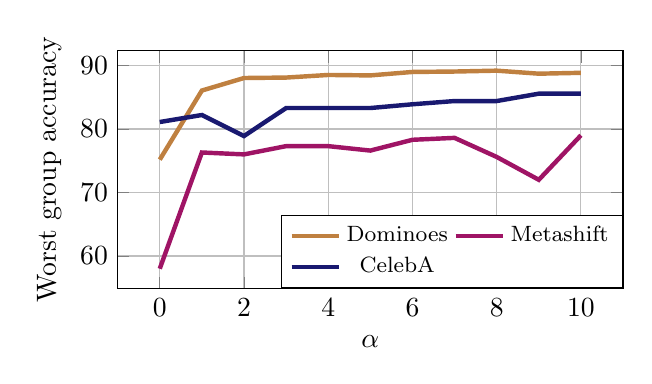
\begin{tikzpicture}
    \begin{axis}[
        xlabel={$\alpha$},
        ylabel={Worst group accuracy},
        legend style={at={(1,0.31)}, legend columns=2,  font=\footnotesize},
        grid=major,
        width=8 cm, height=4.6 cm, every axis plot/.append style={ultra thick}
    ] 
    \addplot[ color=brown] coordinates {
        (0, 75.17 )
        (1, 86.05333333333333)
        (2, 88.02666666666666)
        (3, 88.09666666666667)
        (4, 88.50666666666668)
        (5, 88.43666666666667)
        (6, 88.98)
        (7, 89.04666666666667)
        (8, 89.18333333333334)
        (9, 88.70666666666667)
        (10, 88.84333333333334)
    };
    \addlegendentry{Dominoes}
    %     (0, 75.17 )
    %     (1, 90.95)
    %     (2, 91.75)
    %     (3, 92.06)
    %     (4, 92.21)
    %     (5, 92.68)
    %     (6, 92.68)
    %     (7, 89.04666666666667)
    %     (8, 89.18333333333334)
    %     (9, 88.70666666666667)
    %     (10, 92.83)
    \addplot[color=RedViolet] coordinates {
        (0, 58 )
        (1, 76.3)
        (2, 76)
        (3, 77.3)
        (4, 77.3)
        (5, 76.6)
        (6, 78.3)
        (7, 78.6)
        (8, 75.6)
        (9, 72)
        (10, 79)
    };
    \addlegendentry{Metashift}
    \addplot[color=MidnightBlue] coordinates {
        (0, 81.1 )
        (1, 82.2)
        (2, 78.89)
        (3, 83.3)
        (4, 83.3)
        (5, 83.3)
        (6, 83.89)
        (7, 84.4)
        (8, 84.4)
        (9, 85.56)
        (10, 85.56)
    };
    \addlegendentry{CelebA}
    \end{axis}
\end{tikzpicture}

\end{document}